\chapter{PEMASANGAN TEMPAT SAMPAH}
\label{chap:lampiran-d}

Lampiran ini mendokumentasikan proses pemasangan perangkat \textit{Smart Waste Bin} di lokasi pengujian pada Lantai 4 Gedung Labtek VIII ITB.

\section*{D.1 Pemasangan Roda Tempat Sampah}

\begin{figure}[H]
  \label{fig:lamp-d1}
  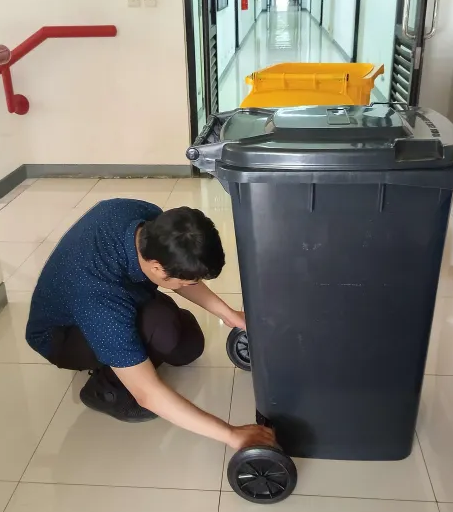
\includegraphics[width=0.75\textwidth]{images/pasang-roda.png}
  \caption{Pemasangan roda pada tempat sampah}
  % RENAME: image32.png → pasang-roda.png
\end{figure}

\section*{D.2 Pemasangan Baterai Perangkat IoT}

\begin{figure}[H]
  \label{fig:lamp-d2}
  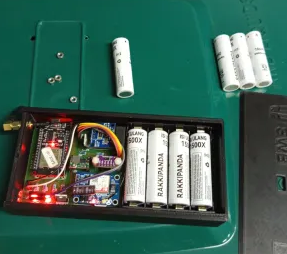
\includegraphics[width=0.65\textwidth]{images/pasang-baterai.png}
  \caption{Pemasangan baterai pada perangkat IoT}
  % RENAME: image33.png → pasang-baterai.png
\end{figure}

\section*{D.3 Pemasangan Perangkat IoT pada Tempat Sampah}

\begin{figure}[H]
  \label{fig:lamp-d3a}
  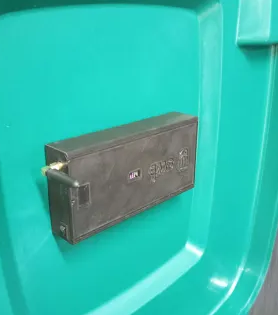
\includegraphics[width=0.65\textwidth]{images/pasang-iot-1.png}
  \caption{Pemasangan perangkat IoT pada tempat sampah (tampak depan)}
  % RENAME: image34.png → pasang-iot-1.png
\end{figure}

\begin{figure}[H]
  \label{fig:lamp-d3b}
  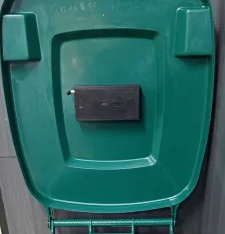
\includegraphics[width=0.65\textwidth]{images/pasang-iot-2.png}
  \caption{Pemasangan perangkat IoT pada tempat sampah (tampak samping)}
  % RENAME: image35.png → pasang-iot-2.png
\end{figure}

\section*{D.4 Pemasangan Label Tempat Sampah}

\begin{figure}[H]
  \label{fig:lamp-d4a}
  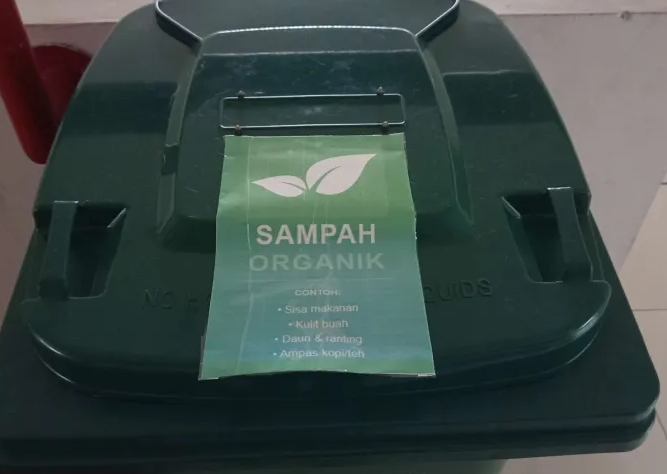
\includegraphics[width=0.75\textwidth]{images/pasang-label-1.png}
  \caption{Pemasangan label tempat sampah organik}
  % RENAME: image36.png → pasang-label-1.png
\end{figure}

\begin{figure}[H]
  \label{fig:lamp-d4b}
  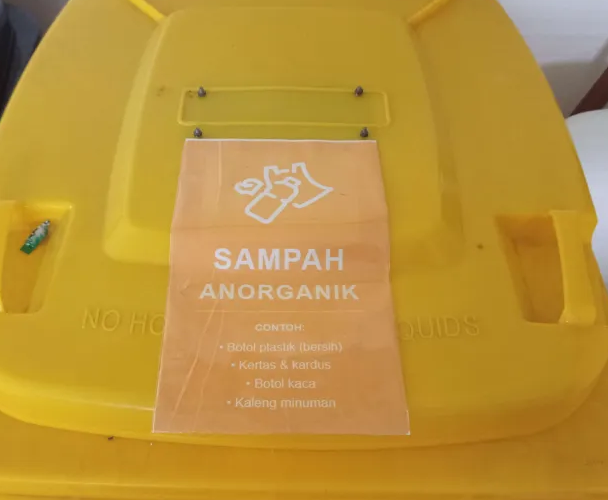
\includegraphics[width=0.75\textwidth]{images/pasang-label-2.png}
  \caption{Pemasangan label tempat sampah anorganik}
  % RENAME: image37.png → pasang-label-2.png
\end{figure}

\begin{figure}[H]
  \label{fig:lamp-d4c}
  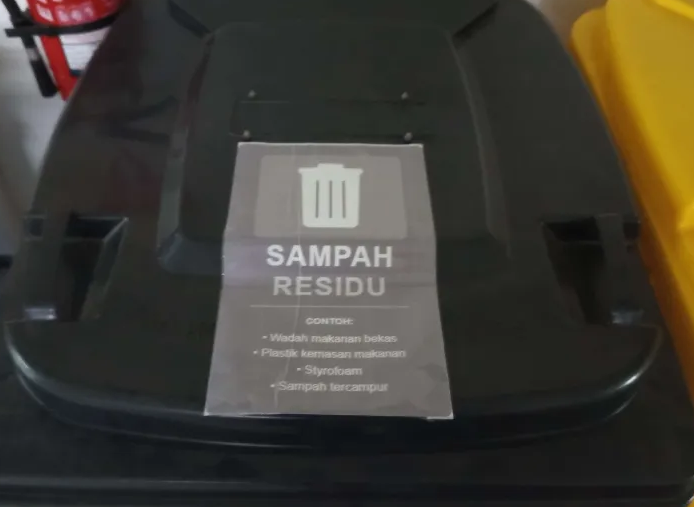
\includegraphics[width=0.75\textwidth]{images/pasang-label-3.png}
  \caption{Pemasangan label tempat sampah residu}
  % RENAME: image38.png → pasang-label-3.png
\end{figure}